% ============================================================
\chapter{Introduction aux EDP}
\label{ch:introduction}
% ============================================================

Les \'equations aux d\'eriv\'ees partielles sont le langage dans lequel la
nature \'ecrit ses lois. L'\'equation de la chaleur d\'ecrit comment la
temp\'erature se diffuse dans un m\'etal. L'\'equation des ondes gouverne la
vibration d'une corde de guitare, la propagation du son, et les ondes
gravitationnelles pr\'edites par Einstein. L'\'equation de Laplace r\`egne sur
l'\'electrostatique, la gravitation newtonienne et les \'ecoulements de
fluides incompressibles. L'\'equation de Schr\"odinger d\'etermine l'\'evolution
de tout syst\`eme quantique.

Ces \'equations, d\'ecouvertes au fil de trois si\`ecles par Euler,
d'Alembert, Fourier, Laplace, et tant d'autres, partagent une
caract\'eristique commune~: elles relient une fonction inconnue de
plusieurs variables \`a ses d\'eriv\'ees partielles. Elles sont plus riches
--- et plus difficiles --- que les \'equations diff\'erentielles ordinaires,
car la multiplicit\'e des variables d'espace et de temps engendre une
vari\'et\'e de comportements~: diffusion, propagation, \'equilibre. Ce premier
chapitre dresse la carte de ce territoire.

% ------------------------------------------------------------
\section{Qu'est-ce qu'une EDP~?}
% ------------------------------------------------------------

Commen\c{c}ons par la d\'efinition la plus g\'en\'erale, avant de sp\'ecialiser.

\begin{definition}[\'Equation aux d\'eriv\'ees partielles]
Une \textbf{\'equation aux d\'eriv\'ees partielles} (EDP) est une \'equation
faisant intervenir une fonction inconnue $u$ de plusieurs variables
ind\'ependantes $(x_1, \ldots, x_n)$ et ses d\'eriv\'ees partielles.
La forme g\'en\'erale est~:
\[
    F\bigl(x_1, \ldots, x_n, u, u_{x_1}, \ldots, u_{x_n},
    u_{x_1 x_1}, u_{x_1 x_2}, \ldots\bigr) = 0.
\]
\end{definition}

\begin{definition}[Ordre d'une EDP]
L'\textbf{ordre} d'une EDP est l'ordre le plus \'elev\'e de d\'erivation
partielle apparaissant dans l'\'equation.
\end{definition}

\begin{exemple}
Quelques EDP classiques~:
\begin{enumerate}
    \item \textbf{\'Equation de transport} (ordre 1)~: $u_t + c\, u_x = 0$.
    \item \textbf{\'Equation de la chaleur} (ordre 2)~: $u_t = k\, u_{xx}$.
    \item \textbf{\'Equation des ondes} (ordre 2)~: $u_{tt} = c^2 u_{xx}$.
    \item \textbf{\'Equation de Laplace} (ordre 2)~: $\Delta u = 0$.
    \item \textbf{\'Equation de Burgers} (ordre 1, non lin\'eaire)~:
          $u_t + u\, u_x = 0$.
    \item \textbf{\'Equation de Korteweg-de Vries} (ordre 3)~:
          $u_t + 6u\, u_x + u_{xxx} = 0$.
\end{enumerate}
\end{exemple}

\section{Lin\'earit\'e et homog\'en\'eit\'e}

\begin{definition}[EDP lin\'eaire]
Une EDP est \textbf{lin\'eaire} si l'op\'erateur $L$ d\'efini par le membre de
gauche est lin\'eaire, c'est-\`a-dire~:
\[
    L(\alpha u + \beta v) = \alpha\, L(u) + \beta\, L(v)
    \quad \forall \alpha, \beta \in \R.
\]
L'EDP est \textbf{homog\`ene} si $Lu = 0$, et \textbf{non homog\`ene} si
$Lu = f$ avec $f \neq 0$.
\end{definition}

\begin{remarque}
Le \textbf{principe de superposition} s'applique aux EDP lin\'eaires homog\`enes~:
si $u_1$ et $u_2$ sont solutions, alors $\alpha u_1 + \beta u_2$ est aussi solution
pour tous $\alpha, \beta \in \R$. Ce principe est fondamental pour la m\'ethode
de s\'eparation des variables.
\end{remarque}

\begin{definition}[EDP semi-lin\'eaire, quasi-lin\'eaire, compl\`etement non lin\'eaire]
\leavevmode
\begin{itemize}
    \item \textbf{Semi-lin\'eaire}~: lin\'eaire dans les d\'eriv\'ees d'ordre le
          plus \'elev\'e, avec coefficients ne d\'ependant que de $x$~:
          $\Delta u = f(x, u, \nabla u)$.
    \item \textbf{Quasi-lin\'eaire}~: lin\'eaire dans les d\'eriv\'ees d'ordre le
          plus \'elev\'e, avec coefficients d\'ependant de $u$ et $\nabla u$~:
          $\sum a_{ij}(x, u, \nabla u)\, u_{x_i x_j} = f(x, u, \nabla u)$.
    \item \textbf{Compl\`etement non lin\'eaire}~: non lin\'eaire dans les
          d\'eriv\'ees d'ordre le plus \'elev\'e~: $\det(D^2 u) = f$ (\'equation
          de Monge-Amp\`ere).
\end{itemize}
\end{definition}

\section{Classification des EDP du second ordre}

Consid\'erons une EDP du second ordre \`a deux variables ind\'ependantes~:
\begin{equation}\label{eq:edp_second_ordre}
    a(x,y)\, u_{xx} + 2b(x,y)\, u_{xy} + c(x,y)\, u_{yy}
    + d(x,y)\, u_x + e(x,y)\, u_y + f(x,y)\, u = g(x,y).
\end{equation}

\begin{definition}[Classification par le discriminant]
Le \textbf{discriminant} de l'EDP \eqref{eq:edp_second_ordre} est
$\Delta_{\mathrm{disc}} = b^2 - ac$. L'EDP est dite~:
\begin{itemize}
    \item \textbf{Elliptique} si $b^2 - ac < 0$ en tout point du domaine.
    \item \textbf{Parabolique} si $b^2 - ac = 0$ en tout point du domaine.
    \item \textbf{Hyperbolique} si $b^2 - ac > 0$ en tout point du domaine.
\end{itemize}
\end{definition}

\begin{intuition}
Cette classification a un sens profond\'ement physique~:
\begin{itemize}
    \item Les EDP \textbf{elliptiques} (type Laplace) mod\'elisent des
          \'etats d'\'equilibre~: la solution en un point d\'epend de la
          solution partout autour.
    \item Les EDP \textbf{paraboliques} (type chaleur) mod\'elisent des
          processus de diffusion~: l'information se propage \`a vitesse
          infinie mais s'att\'enue.
    \item Les EDP \textbf{hyperboliques} (type ondes) mod\'elisent des
          ph\'enom\`enes de propagation~: l'information se propage \`a vitesse finie
          le long de caract\'eristiques.
\end{itemize}
\end{intuition}

\begin{exemple}
\leavevmode
\begin{enumerate}
    \item $u_{xx} + u_{yy} = 0$ (Laplace)~: $a = 1$, $b = 0$, $c = 1$,
          donc $b^2 - ac = -1 < 0$~: \textbf{elliptique}.
    \item $u_t - u_{xx} = 0$ (chaleur)~: $a = -1$, $b = 0$, $c = 0$,
          donc $b^2 - ac = 0$~: \textbf{parabolique}.
    \item $u_{tt} - c^2 u_{xx} = 0$ (ondes)~: $a = -c^2$, $b = 0$, $c_{\text{coeff}} = 1$,
          donc $b^2 - ac = c^2 > 0$~: \textbf{hyperbolique}.
\end{enumerate}
\end{exemple}

\subsection{Classification en dimension sup\'erieure}

Pour une EDP du second ordre \`a $n$ variables~:
\[
    \sum_{i,j=1}^{n} a_{ij}(x)\, u_{x_i x_j}
    + \text{termes d'ordre inf\'erieur} = 0,
\]
la classification repose sur la \textbf{matrice des coefficients}
$A = (a_{ij})$, suppos\'ee sym\'etrique~:
\begin{itemize}
    \item \textbf{Elliptique}~: toutes les valeurs propres de $A$ sont de m\^eme signe.
    \item \textbf{Hyperbolique}~: une valeur propre de signe oppos\'e aux autres.
    \item \textbf{Parabolique}~: une valeur propre nulle, les autres de m\^eme signe.
\end{itemize}

\begin{theoreme}[Forme canonique --- cas $n=2$]
Par un changement de variables $(\xi, \eta) = (\xi(x,y), \eta(x,y))$
bien choisi, toute EDP lin\'eaire du second ordre \`a deux variables peut
\^etre ramen\'ee \`a l'une des formes canoniques suivantes~:
\begin{itemize}
    \item \textbf{Elliptique}~: $u_{\xi\xi} + u_{\eta\eta} + \cdots = 0$.
    \item \textbf{Parabolique}~: $u_{\xi\xi} + \cdots = 0$.
    \item \textbf{Hyperbolique}~: $u_{\xi\xi} - u_{\eta\eta} + \cdots = 0$
          ou de mani\`ere \'equivalente $u_{\alpha\beta} + \cdots = 0$ avec
          $\alpha = \xi + \eta$, $\beta = \xi - \eta$.
\end{itemize}
\end{theoreme}

\section{Conditions aux limites et conditions initiales}

\begin{definition}[Probl\`eme aux limites]
Un \textbf{probl\`eme aux limites} consiste en une EDP pos\'ee sur un domaine
$\Omega \subset \R^n$ compl\'et\'ee par des conditions sur la fronti\`ere
$\partial\Omega$. Les types principaux sont~:
\begin{enumerate}
    \item \textbf{Dirichlet}~: $u = g$ sur $\partial\Omega$.
    \item \textbf{Neumann}~: $\frac{\partial u}{\partial \nu} = g$ sur
          $\partial\Omega$, o\`u $\nu$ est la normale ext\'erieure.
    \item \textbf{Robin} (mixte)~: $\alpha u + \beta \frac{\partial u}{\partial \nu} = g$
          sur $\partial\Omega$.
\end{enumerate}
\end{definition}

\begin{center}
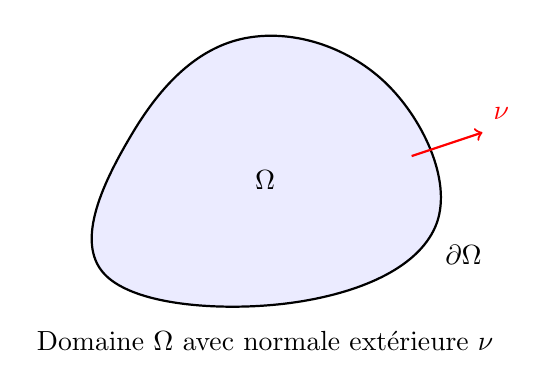
\begin{tikzpicture}[scale=1.2]
    % Domaine
    \draw[thick, fill=blue!8] plot[smooth cycle, tension=0.7]
        coordinates {(0,0) (2,-0.3) (3.5,0.5) (3,2) (1.5,2.5) (0.3,1.5)};
    \node at (1.7,1) {$\Omega$};
    % Normale
    \draw[->, thick, red] (3.25,1.25) -- (4.0,1.5);
    \node[red] at (4.2,1.7) {$\nu$};
    % Labels
    \node at (3.8,0.2) {$\partial\Omega$};
    % Points
    \node[below] at (1.7, -0.5) {Domaine $\Omega$ avec normale ext\'erieure $\nu$};
\end{tikzpicture}
\end{center}

\begin{definition}[Probl\`eme bien pos\'e au sens de Hadamard]
Un probl\`eme est dit \textbf{bien pos\'e} au sens de Hadamard s'il
v\'erifie les trois conditions suivantes~:
\begin{enumerate}
    \item \textbf{Existence}~: il existe au moins une solution.
    \item \textbf{Unicit\'e}~: il existe au plus une solution.
    \item \textbf{Stabilit\'e}~: la solution d\'epend continûment des donn\'ees.
\end{enumerate}
\end{definition}

\begin{attention}[title=\textbf{Importance du caract\`ere bien pos\'e}]
Un probl\`eme mal pos\'e n'est pas n\'ecessairement sans int\'er\^et
math\'ematique ou physique. L'exemple classique de Hadamard montre que le
probl\`eme de Cauchy pour l'\'equation de Laplace est mal pos\'e, mais des
techniques de r\'egularisation permettent de l'aborder.
\end{attention}

\begin{exemple}[Probl\`eme de Dirichlet pour le laplacien sur le disque]
Trouver $u$ harmonique dans le disque unit\'e $D = \{(x,y) : x^2+y^2 < 1\}$
avec $u = g$ sur $\partial D = \{x^2+y^2=1\}$. En coordonn\'ees polaires~:
\[
    \begin{cases}
        u_{rr} + \frac{1}{r}u_r + \frac{1}{r^2}u_{\theta\theta} = 0,
        & 0 < r < 1,\\
        u(1,\theta) = g(\theta).
    \end{cases}
\]
Ce probl\`eme est bien pos\'e (existence, unicit\'e, stabilit\'e).
\end{exemple}

\section{Probl\`emes d'\'evolution}

\begin{definition}[Probl\`eme de Cauchy]
Pour une EDP d'\'evolution (parabolique ou hyperbolique), le \textbf{probl\`eme
de Cauchy} consiste \`a trouver $u(x,t)$ v\'erifiant l'EDP pour $t > 0$ et
des \textbf{conditions initiales} pour $t = 0$~:
\begin{itemize}
    \item Pour l'\'equation de la chaleur~: $u(x,0) = u_0(x)$.
    \item Pour l'\'equation des ondes~: $u(x,0) = u_0(x)$ et $u_t(x,0) = v_0(x)$.
\end{itemize}
\end{definition}

\begin{center}
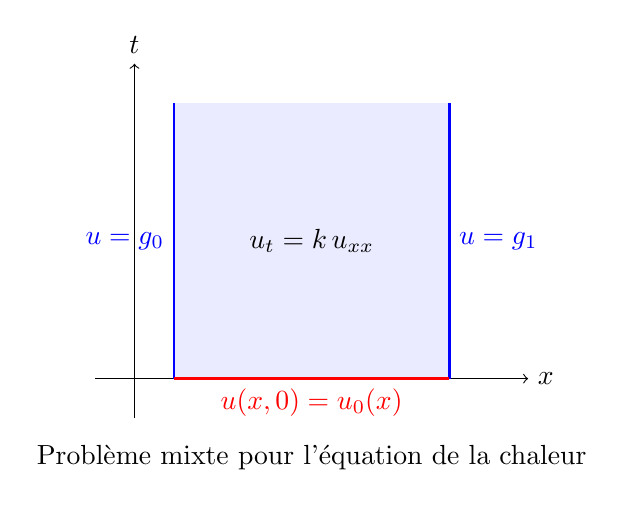
\begin{tikzpicture}[scale=1.0]
    % Axes
    \draw[->] (-0.5,0) -- (5,0) node[right] {$x$};
    \draw[->] (0,-0.5) -- (0,4) node[above] {$t$};
    % Domaine espace-temps
    \fill[blue!8] (0.5,0) rectangle (4,3.5);
    \draw[thick, blue] (0.5,0) -- (0.5,3.5);
    \draw[thick, blue] (4,0) -- (4,3.5);
    \draw[very thick, red] (0.5,0) -- (4,0);
    % Labels
    \node[red, below] at (2.25,0) {$u(x,0) = u_0(x)$};
    \node[blue, left] at (0.5,1.75) {$u=g_0$};
    \node[blue, right] at (4,1.75) {$u=g_1$};
    \node at (2.25,1.75) {$u_t = k\,u_{xx}$};
    \node at (2.25, -1) {Probl\`eme mixte pour l'\'equation de la chaleur};
\end{tikzpicture}
\end{center}

\section{Exemples fondamentaux de mod\'elisation}

\subsection{D\'erivation de l'\'equation de la chaleur}

Consid\'erons une barre mince de longueur $L$. Soit $u(x,t)$ la temp\'erature
au point $x \in [0,L]$ \`a l'instant $t$. La conservation de l'\'energie sur
un segment $[a,b]$ donne~:
\[
    \frac{d}{dt}\int_a^b \rho\, c_p\, u(x,t)\,dx
    = -q(a,t) + q(b,t) + \int_a^b f(x,t)\,dx,
\]
o\`u $\rho$ est la densit\'e, $c_p$ la capacit\'e thermique, $q$ le flux
de chaleur et $f$ un terme source. La loi de Fourier donne
$q(x,t) = -k\, u_x(x,t)$. En d\'erivant sous le signe int\'egral~:
\[
    \int_a^b \rho\, c_p\, u_t\, dx = \int_a^b k\, u_{xx}\, dx
    + \int_a^b f\, dx.
\]
Comme ceci vaut pour tout $[a,b]$, on obtient~:
\[
    \rho\, c_p\, u_t = k\, u_{xx} + f,
\]
soit, en posant $\kappa = k/(\rho c_p)$~:
\begin{equation}\label{eq:chaleur_derivation}
    u_t = \kappa\, u_{xx} + \tilde{f}.
\end{equation}

\subsection{D\'erivation de l'\'equation des ondes}

Consid\'erons une corde vibrante de densit\'e lin\'eaire $\rho$ soumise
\`a une tension $T$. Pour de petits d\'eplacements transversaux $u(x,t)$,
le principe fondamental de la dynamique appliqu\'e \`a un \'el\'ement
$[x, x+dx]$ donne~:
\[
    \rho\, dx\, u_{tt} = T\sin\theta(x+dx) - T\sin\theta(x)
    \approx T\bigl(u_x(x+dx) - u_x(x)\bigr) = T\, u_{xx}\, dx.
\]
On obtient donc~:
\begin{equation}\label{eq:ondes_derivation}
    u_{tt} = c^2\, u_{xx}, \quad c = \sqrt{T/\rho}.
\end{equation}

\section{Exemples de solutions explicites}

\begin{exemple}[Solutions de l'\'equation de Laplace en 2D]
Les fonctions harmoniques suivantes sont solutions de $\Delta u = 0$
dans $\R^2$~:
\begin{enumerate}
    \item $u(x,y) = ax + by + c$ (fonctions affines).
    \item $u(x,y) = x^2 - y^2$ (v\'erification~: $u_{xx} + u_{yy} = 2 - 2 = 0$).
    \item $u(x,y) = e^x \cos y$ (v\'erification~: $u_{xx} + u_{yy} = e^x\cos y - e^x\cos y = 0$).
    \item $u(r,\theta) = r^n \cos(n\theta)$ en polaires, pour tout $n \in \N$.
\end{enumerate}
\end{exemple}

\begin{exemple}[Ondes progressives]
La fonction $u(x,t) = f(x - ct)$ est solution de l'\'equation des ondes
$u_{tt} = c^2 u_{xx}$ pour toute fonction $f$ de classe $C^2$. En effet~:
\[
    u_t = -c f'(x-ct), \quad u_{tt} = c^2 f''(x-ct), \quad
    u_x = f'(x-ct), \quad u_{xx} = f''(x-ct).
\]
Donc $u_{tt} = c^2 u_{xx}$. De m\^eme, $g(x+ct)$ est solution (onde se
propageant vers la gauche).
\end{exemple}

\section{Notion de solution}

\begin{definition}[Solution classique]
Une \textbf{solution classique} d'une EDP d'ordre $k$ est une fonction
$u \in C^k(\Omega)$ qui satisfait l'EDP en tout point de $\Omega$.
\end{definition}

\begin{definition}[Solution faible]
Une \textbf{solution faible} est une fonction $u$ appartenant \`a un espace
fonctionnel ad\'equat (par exemple un espace de Sobolev) qui satisfait
l'EDP au sens des distributions, c'est-\`a-dire~:
\[
    \int_\Omega u\, L^*\varphi\, dx = \int_\Omega f\, \varphi\, dx
    \quad \forall \varphi \in C_c^\infty(\Omega),
\]
o\`u $L^*$ est l'adjoint formel de l'op\'erateur $L$.
\end{definition}

\begin{remarque}
La notion de solution faible est essentielle pour les raisons suivantes~:
\begin{enumerate}
    \item Certaines EDP n'admettent pas de solution classique (par exemple
          les lois de conservation hyperboliques d\'eveloppent des chocs).
    \item Le cadre faible permet d'utiliser les outils de l'analyse fonctionnelle
          (th\'eor\`eme de Lax-Milgram, m\'ethodes variationnelles).
    \item Sous des hypoth\`eses de r\'egularit\'e, on peut souvent montrer qu'une
          solution faible est en fait classique.
\end{enumerate}
\end{remarque}

\section{Exercices}

\begin{exercice}
Classifier les EDP suivantes (elliptique, parabolique, hyperbolique)~:
\begin{enumerate}
    \item $u_{xx} + 2u_{xy} + u_{yy} = 0$.
    \item $u_{xx} + 2u_{xy} + 5u_{yy} = 0$.
    \item $3u_{xx} - 4u_{xy} + u_{yy} = 0$.
    \item $u_{xx} + x^2 u_{yy} = 0$ (le type d\'epend-il de $x$~?).
\end{enumerate}
\end{exercice}

\begin{exercice}
Montrer que la superposition $u = \sum_{k=1}^{N} c_k u_k$ de solutions
d'une EDP lin\'eaire homog\`ene est encore solution. Ce r\'esultat
s'\'etend-il au cas non homog\`ene~?
\end{exercice}

\begin{exercice}
V\'erifier que $u(x,y) = \ln(x^2 + y^2)$ est harmonique dans
$\R^2 \setminus \{0\}$. Calculer $\nabla u$ et interpr\'eter
physiquement cette solution.
\end{exercice}

\begin{exercice}
D\'eriver l'\'equation de la chaleur en dimension $n$~:
\[
    u_t = \kappa\, \Delta u + f
\]
en utilisant la conservation de l'\'energie et la loi de Fourier
$\vec{q} = -k \nabla u$ dans un domaine arbitraire $\Omega \subset \R^n$.
\end{exercice}

\begin{exercice}[Probl\`eme de Hadamard]
Consid\'erer le probl\`eme de Cauchy pour l'\'equation de Laplace~:
\[
    u_{xx} + u_{yy} = 0, \quad u(x,0) = 0, \quad
    u_y(x,0) = \frac{1}{n}\sin(nx).
\]
Montrer que la solution est $u(x,y) = \frac{1}{n^2}\sin(nx)\sinh(ny)$.
En d\'eduire que lorsque $n \to \infty$, la donn\'ee initiale tend vers $0$
uniform\'ement mais la solution ne tend pas vers $0$ pour $y \neq 0$.
Conclure sur le caract\`ere mal pos\'e.
\end{exercice}

\begin{exercice}
Soit l'\'equation de Tricomi~: $u_{xx} + y\, u_{yy} = 0$.
D\'eterminer les r\'egions du plan o\`u cette EDP est elliptique,
parabolique ou hyperbolique. Tracer ces r\'egions.
\end{exercice}
